\chapter{Control}
\label{chap:control}

\section{Overview of the control system}
This is an overview of the information flow for control in regard to the rest of the system containing, sensors, \ac{LLI} and \ac{HLI}.

\begin{figure}[htbp]
	\centering
	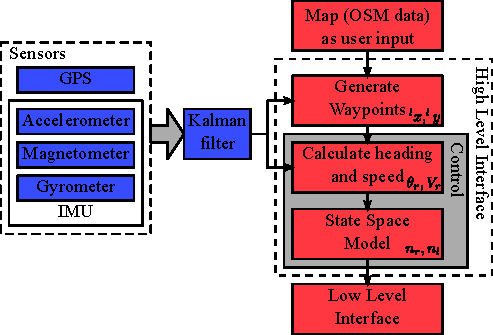
\includegraphics[width=\textwidth]{img/vessel-block-overview}
	\caption{Overview of control information flow in regard to the subsystems. The blue part indicates information that is not fetched fed to the control part, it is electrically connected to the \ac{LLI} whilst being forwarded to the \ac{HLI}. The red parts is what happens on the \ac{HLI}. The yellow part is the \ac{LLI} itself.}
	\label{fig:vessel-block-overview}
\end{figure}

\todo{Illustrate on figure~\vref{fig:vessel-block-overview} where RF comms is or maybe that should be on the block overvieww diagram without regard to contorl abstraction}



In the First Stage the required heading of the ship is calculated that keeps the course closest to the planned waypoint.

In order to efficiently and accurately navigate along the path, a set of Sub-Waypoints is calculated for each route between two Waypoints. The main control strategy is to navigate through all of these SWPs in a predefined order, one by one. (Navigation Figure) The heading of the ship is defined in NED coordinate system. The required heading is determined by the Law of Cosines, based on the Position of the Ship and the Position of the next Sub-Waypoint.
\begin{center}
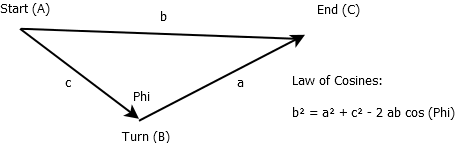
\includegraphics[scale = 0.4]{img/ControlStrategyFigures/Law_of_Cosines.png}
\end{center}
Problems rise and corrections are necessary, if the heading of the ship $\theta$ is $\theta < -\pi$ or $\theta < \pi$. The heading of the ship is calculated based on the Gyro sensor and the heading can have any value in the form of: $$\theta = [-{\pi} ; \pi ] \pm 2 \cdot k \cdot \pi$$. Before invoking the control procedure, all of the heading angles must be transformed into the $[-\pi ; \pi]$ interval.
This procedure causes a possible error though.

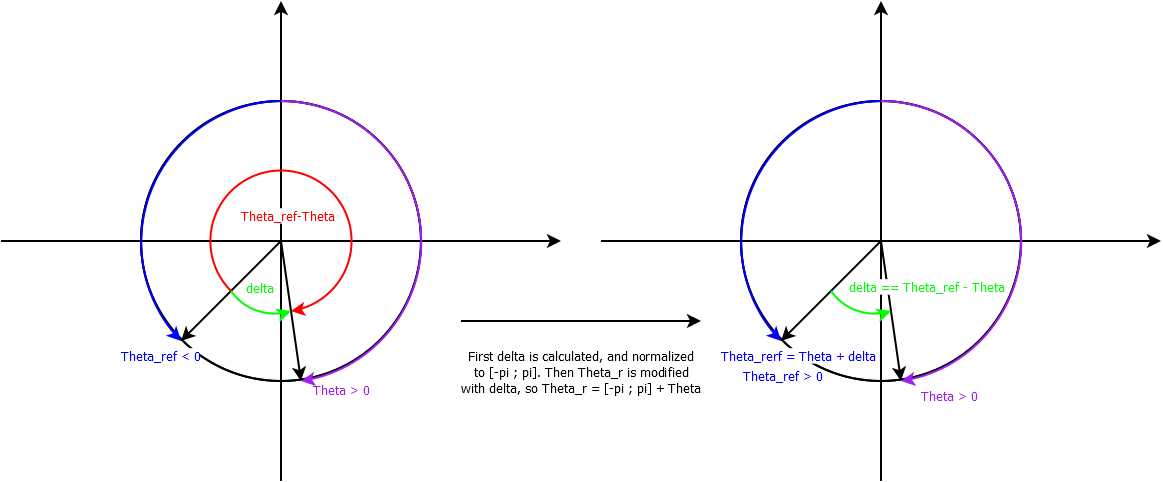
\includegraphics[width=\textwidth]{img/ControlStrategyFigures/Headings.png}

The required heading or the heading of the ship must be transformed into a different representation, where $$|\theta_{r}-\theta| < \pi$$. To keep a consistent heading representation, first the deviation angle $$\theta = \pi_{r}-\pi$$ is calculated, than transformed to the $[-\pi;\pi]$ interval and finally, with $\delta$ we can transform $\theta_{r}$ to $$\theta_{r}(\theta) = \theta + \delta$$.
If the conditions above are met, $\theta$ and $\theta_r(\theta)$ will always yield values that result in correct controller output.

\subsection{Subwaypoint Validity}

The overall navigation can be improved, if the Target SWPs are considered ``reached'' in a certain distance. Optimally this distance (Validity distance) should be somewhat longer than the minimum turning radius of the ship ($R_{min}$). If it is shorter, the ship might not be able to reach the SWP, if it is way longer, the ship will divert from its course in turns.

\section{Control loop theory}

The inner control is implemented by a State-Space controller, based on the difference of the estimated and the reference states, speed and heading:
\begin{align}
Q = F(X-\hat{x}) \quad , \quad x = [v, \theta]^T
\end{align}

\subsection{Linearizing the outputs}

Using Newton's second law of motion for forward  and rotational movement ($F = m \cdot A$ and $T = I \cdot \dot{\omega}$), we can easily see that the inputs to our system will be F and T representing the forward force and the torque produced by the motors. It is worth mentioning that, since there are two propellers rotating in opposite directions, a torque that would induce a rotation around Z axis passing through the boat's center of mass only if the two propellers are rotating at different speeds.

These two rotational speeds N1 and N2 were initially included in the state space model as inputs to the system, as they could be controlled directly via a PWM pulse. This though proved to complicate matters because the relationship between the speeds of the propellers N1 and N2 and the force F and torque T generating accelerations is not a linear one. Because of this, our system would not be linear and would be beyond the scope of this project. 

\todo{insert formulas for [F, T] -> [n1, n2] transformation here}

In order to prevent this from happening, the state space model was updated to only calculate the force T and torque T necessary for driving and turning the ship, and this would keep our system linear. in order to transform from [T, F] to [N1, N2], another module was introduced in the system which would implement this non-linear function. 

This is a better solution anyway because if the state space model only outputs T and F, then it could be used for some other ship configurations, without modifications to the model, only to the module that translates the force and torque to N1 and N2. This, for example, can allow us to change the size of the propellers or their positions.

\subsection{Linearizing the drag forces}
\label{sect:Linearizing drag forces}

The drag forces acting on the bow of the ship while it's moving through the water are influenced by the area of the hull that is below water depth in the direction of movement, the density of the water, a drag constant $ C_{D} $ , and the square of the ship's speed components $ v_{x} $ and $ v_{y} $. 

A worthy note is the fact that the drag coefficient $ C_{D} $ will have two values depending on the direction of the ship's movement. When moving forward in the $x$ direction, the coefficient $ C_{Dx} $ will be approximated for a triangular shape, which is the closest simple shape that we have values for. For lateral movement in the $y$ direction, $ C_{Dy} $ is given for a square box. These approximations should not present a problem in the operation of our control system as the errors ca easily be corrected and adjusted for by a good controller.

\[ D_{x}(v_{x}) = \frac{C_{Dx}\cdot\rho_{water}\cdot A_{front}\cdot v_{x}^{2}}{2} \]
\[ D_{y}(v_{y}) = \frac{C_{Dy}\cdot\rho_{water}\cdot A_{side}\cdot  v_{y}^{2}}{2} \]

Where $ D_{x}(v_{x}) $ and $ D_{y}(v_{y})$ are the drag forces dependent on the forward and lateral speeds respectively, $ \rho_{water} $ is the density of the water, $ A_{front} $ is the frontal area of the hull and $ A_{side} $ is the lateral area. 

The drag torque that is produced by the drag force acting on the hull of the ship, as the ship rotates through the water is dependent on the square of the angular velocity $ \omega $:

\[ \tau(\omega) = \frac{C_{D} \cdot \rho_{water} \cdot d \cdot (r_{f}^{4} + r_{b}^{4}) \cdot \omega^{2}}{8} \]

Where $ \tau(\omega) $ is the torque generated by the angular speed $ \omega $, $ d  $ is the depth of the ship that is submerged in water, $ r_{f} $ and $ r_{b} $ are the radii of the ship from the center of mass towards the front and back end, respectively.

These forces are obviously non-linear and thus cannot be integrated into the linear Kalman filter or State Space Model. Because we will usually use a constant speed it is feasible to linearize these forces for that value and not have big errors. The angular drag torque can also be linearized around a mean turning speed because the radii of the corners of the paths are also constant.

Approximation of the drag forces around the points of interest $v_{l} $ and $\omega_{l}$ is done using the first order term of the Taylor expansion:

\[ y_{l}(x) = f(a) + f'(a)(x-a) \]

Where $y = f(x)$ is the function we want to linearize around a value of interest $a$. Applying this formula to our situation yields:

\[ Dx_{l}(v_{x}) = \frac{C_{Dx}\cdot\rho_{water}\cdot A_{front}\cdot v_{l}^{2}}{2} + (C_{Dx}\cdot\rho_{water}\cdot A_{front})\cdot (v_{x}-v_{l}) \]

\[ Dy_{l}(v_{y}) = \frac{C_{Dy}\cdot\rho_{water}\cdot A_{side}\cdot v_{l}^{2}}{2} + (C_{Dy}\cdot\rho_{water}\cdot A_{side})\cdot (v_{y}-v_{l}) \]

\[ \tau_{l}(\omega) = \frac{C_{Dy} \cdot \rho_{water} \cdot d \cdot (r_{f}^{4} + r_{b}^{4}) \cdot \omega_{l}^{2}}{8} + \frac{C_{Dy} \cdot \rho_{water} \cdot d \cdot (r_{f}^{4} + r_{b}^{4}) \cdot \omega_{l}}{4} \cdot (\omega - \omega_{l}) \] 

\begin{figure}[htbp]
	\centering
	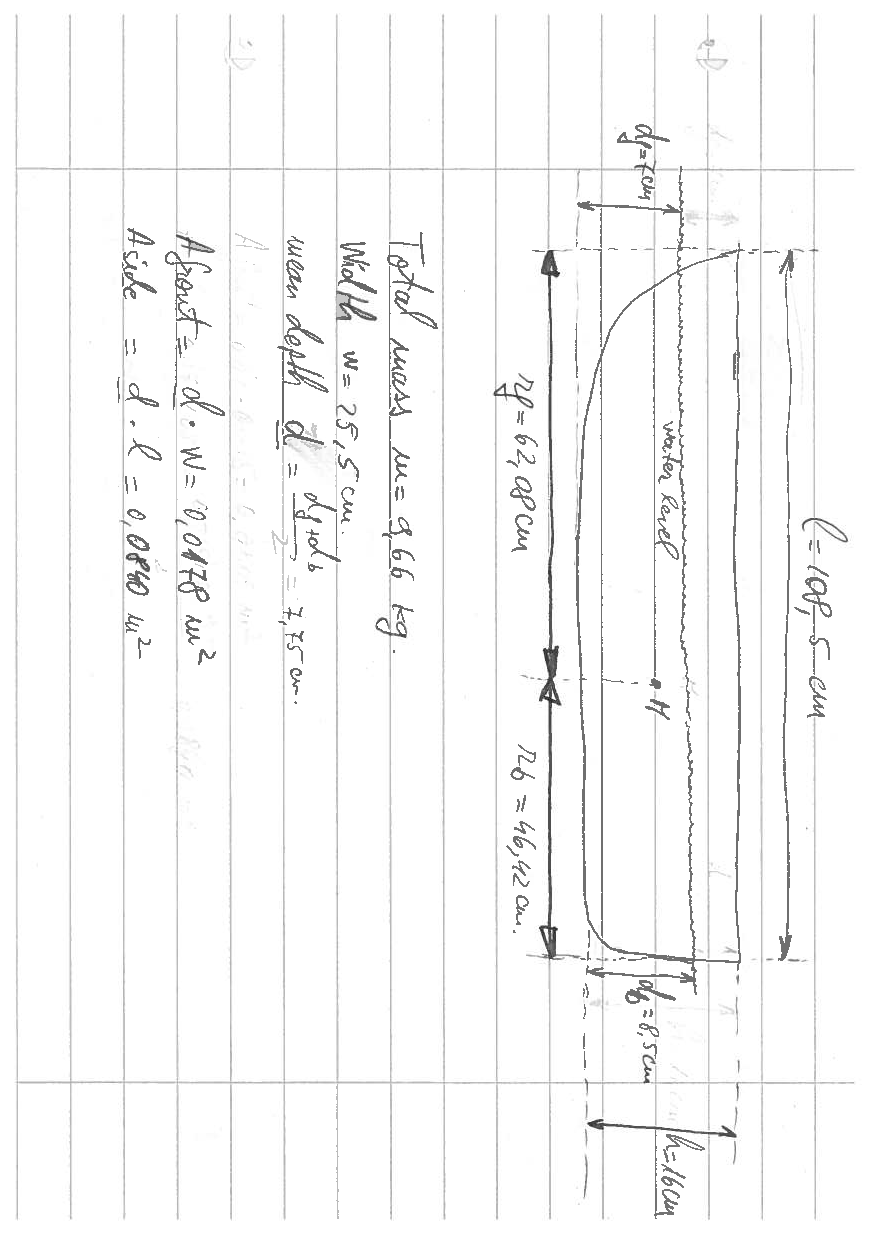
\includegraphics[width=\textwidth, trim=1.8cm 0cm 0cm 2cm, clip = true, angle = 90, width=\textwidth]{img/ship_sizes}
	\caption{Sketch of ship sizes as measured after the maiden voyage}
	\label{fig:ship_sizes}
\end{figure}

Given figure \vref{fig:ship_sizes}:
 $ v_{l} = 1m/s $ , \quad
 $ \omega_{l} = 1 s ^{-1} $ ,\quad
 $ C_{Dx} = 0.5 $ (triangle) ,\quad
 $ C_{Dy} = 1 $ (box) ,\quad
 $ \rho = 1000 kg/m ^{2} $,\quad
 $ A_{front} = 0.0178 m^{2} $,\quad
 $ A_{side} = 0.0840 m ^{2} $,\quad
 $ d = 0.0775 m $,\quad
 $ r_{f} = 0.6208 m $,\quad
 $ r_{b} = 0.4642 m $,\quad
the linearized formulas for the drag forces can be computed to be:


\begin{align}
 Dx_{l}(v) &= -4.45 + 8.9 \cdot v_{x} \\
 Dy_{l}(v) &= -42 + 84 \cdot v_{y} \\
 \tau_{l}(\omega) &= -1.88 + 3.77 \cdot \omega
\end{align}

From which we can identify the coefficients that correspond tot the linear relation $ y_{l}(x) = \alpha + \beta \cdot x $:\\
\begin{minipage}{0.3\linewidth}
\[ \alpha_{x} = -4.45 \]
\[ \beta_{x} = 8.9 \]
\end{minipage}
\begin{minipage}{0.3\linewidth}
\[ \alpha_{y} = -42 \] 
\[ \beta_{y} = 84 \]
\end{minipage}
\begin{minipage}{0.3\linewidth}
\[ \alpha_{\omega} = -1.88 \]
\[ \beta_{\omega} = 3.77 \]
\end{minipage}


\subsection{Choosing the right states}

The variables we chose to be the states in our model are the speed of the ship in the forward direction in the ship frame $v$, the angular position of the ship's x axis relative to true North $\theta$ and the angular speed $\omega$.\\
\begin{align}\begin{cases}
F - F_{D} = m \cdot \dot{v}\\
T - T_{D} = I \cdot \dot{\omega}\\
\end{cases}\end{align}

Where $ F $ and $ T $ are the force and torque produced by the propellers, $ F_{D} $ and $ T_{D} $ are the force and torque caused by water drag, $ m $ is the mass of the ship, $ I $ is the moment of inertia, $ \dot{v} $  and $ \dot{\omega} $ are forward and angular acceleration respectively.

The linearized drag force and torque from \ref{sect:Linearizing drag forces} can be substituted in these equations:
\begin{align}
 \dot{v} &= \frac{1}{m}(- \beta_{x} \cdot v + \vec{F})\\
 \dot{\omega} &= \frac{1}{I}(-\beta_{y} \cdot \omega + T)\\
 \dot{\theta} &= \omega
\end{align}

Note that we have also dropped the $ \alpha $ term of the equations because we're currently only interested in the dynamic behavior of the system. The $ \alpha $ offset will be compensated for when removing the steady state error. Consequently, these relations can be rewritten in a matrix notation as follows:
\begin{align}
\dot{
	\begin{bmatrix}
	 v\\
	 \theta\\
	 \omega
	\end{bmatrix}
}
=
\begin{bmatrix}
 -\frac{\beta_{x}}{m} & 0 & 0\\
 0 & 0 & 1\\
 0 & 0 & - \frac{\beta_{y}}{I}\\
\end{bmatrix}
\cdot
\begin{bmatrix}
v\\
\theta\\
\omega
\end{bmatrix}
+
\begin{bmatrix}
\frac{1}{m} & 0\\
0 & 0\\
0 & \frac{1}{I}\\
\end{bmatrix}
\cdot
\begin{bmatrix}
F\\
T
\end{bmatrix}
\label{eq:ssmodel}
\end{align}
Equation \vref{eq:ssmodel} corresponds to a 3 \ac{DOF} model for the ship - with the 3 degrees noted as movement in the X-direction ($x$), Y-direction ($y$) and the rotation about the Z-axis ($\theta$). This model corresponds to the state equations, which are used as a base for developing the control algorithm.
\begin{align}
\vec{\dot{x}} = \vec{A}\vec{x} + \vec{B}\vec{u}
\end{align}
Since we only need to output the velocity and the angle, the output matrix $\vec{C}$ is added to the system. No feedforward loop is implemented, so this part can be removed, resulting in the output equation for the system becomes:
\begin{align}
\vec{y} = \vec{C}\vec{x}
\end{align}

\subsection{Discretizing for use with a particular timestep}

The system described so far is continuous and needs to be discretized before being converted into an algorithm. Discretization is carried out in \MATLAB \ using the \texttt{c2d} command. This command takes the continous time state space model and the discretization time step - and outputs the discrete equivalent. The \texttt{c2d} command uses a zero-order hold algorithm to discretize the system.
The zero order hold algorithm is defined as:
\begin{align}
\vec{x}(t)  = \sum_{n = -\infty}^{\infty} \vec{x}[n] \cdot \text{rect}\left(\frac{t-T/2 - nT}{T}\right)
\end{align}
\noindent Where:
\begin{ffk}
$\text{rect}$ is a rectangular window function\\
$T$ is the time interval
\end{ffk}
The matrices once discretized becomes:
\begin{align}
\dot{
	\begin{bmatrix}
	 v(k)\\
	 \theta(k)\\
	 \omega(k)
	\end{bmatrix}
}
=
\begin{bmatrix}
 -\frac{\beta_{x}}{m} & 0 & 0\\
 0 & 0 & 1\\
 0 & 0 & - \frac{\beta_{y}}{I}\\
\end{bmatrix}
\begin{bmatrix}
v(k-1)\\
\theta(k-1)\\
\omega(k-1)
\end{bmatrix}
+
\begin{bmatrix}
\frac{1}{m} & 0\\
0 & 0\\
0 & \frac{1}{I}\\
\end{bmatrix}
\begin{bmatrix}
F(k)\\
T(k)
\end{bmatrix}
\label{eq:ssmodel}
\end{align}

\subsection{Optimal pole assignment}
To achieve an optimal response of the system, an optimal pole placement strategy have been used. This is done by minimizing the cost function in equation \vref{eq:optf}. The optimal pole placement is then computed by solving the Algebraic Ricatti Equation. 
\begin{align}
\mathcal{J}(u)=\int_{0}^{\infty} (\vec{x}^T \vec{Q} \vec{x} + \vec{u}^T \vec{R} \vec{u}) dt
\label{eq:optf}
\end{align}
Again, this is done in \MATLAB, and gives poles in:
\todo{insert poles once final -lunde}
\begin{align}
\vec{F}_{opt} = \begin{bmatrix}
0 & 0 & 0\\
0 & 0 & 0
\end{bmatrix}
\end{align}
This changes the input of the system to $\vec{u} = -\vec{F}_{opt}\vec{x}$, however, this does not take into account that we can end up with a steady state error. Therefore a reference gain is introduced. 


\subsection{Reference gain}
The purpose of the reference gain is to zero out the steady state error. This is done by augmenting the state space system, and equating the error to zero. This can be written as:
\begin{align}
\vec{0} &= \vec{A}\vec{x}_{ss} + \vec{G}\vec{u}_{ss}\\
\vec{y}_{ss} &= \vec{C}\vec{x}_{ss} + \vec{D}\vec{u}_{ss}
\end{align}
The gain $N$ is now introduced as a scaling factor on the reference signal, to make this error zero. The input $\vec{u}$ of the steady state version is then changed to the reference signal multiplied with the steady state input of the system. Written on matrix form this becomes:
\begin{align}
\begin{bmatrix}
\vec{A} & \vec{B}\\
\vec{C} & \vec{D}
\end{bmatrix}\begin{bmatrix}
\vec{N}_x\\
\vec{N}_u
\end{bmatrix} = \begin{bmatrix}
\vec{0}\\
\vec{I}
\end{bmatrix}
\end{align}
Thus, solving for $\begin{bmatrix} \vec{N}_x\\ \vec{N}_u \end{bmatrix}$ gives the following: \todo{insert refference to feedback book, page 470}
\begin{align}
\begin{bmatrix}
\vec{N}_x\\
\vec{N}_u
\end{bmatrix} =
\begin{bmatrix}
\vec{A} & \vec{B}\\
\vec{C} & \vec{D}
\end{bmatrix}^{-1}
\begin{bmatrix}
0\\
\vec{I}
\end{bmatrix}
\end{align}
Thus the final control signal changing the input $\vec{u}$ to:
\begin{align}
\vec{u} = -\vec{F}_{opt}\vec{x} + (\vec{N}_u + \vec{F}_{opt}\vec{N}_{\vec{x}})\vec{r}
\label{eq:refg}
\end{align}
The latter in equation \vref{eq:refg} can be combined, and gives the following:
\begin{align}
\vec{u} = -\vec{F}_{opt}\vec{x} + \bar{\vec{N}}\vec{r}
\end{align}


\section{Implementation of control loop}

The control loop is implemented in Python and is run on the HLI.

The control loop reads the data from the LLI communication and invokes the control function of the Ship Object at every timestep.

(Figure!)

The control function of the Ship Object processes the data sent by the LLI. The data is a 9-by-2 matrix, which consists of the measurement values and the validity of the measurements. A measurement is considered valid, if its validity value is 1.

\begin{align}
M_{[9,2]} =
  \begin{pmatrix}
   M_1 & V_1 \\
   M_2 & V_2 \\
   M_3 & V_3 \\
   M_4 & V_4 \\
   M_5 & V_5 \\
   M_6 & V_6 \\
   M_7 & V_7 \\
   M_8 & V_8 \\
   M_9 & V_9
  \end{pmatrix}
\end{align}

We can process this matrix to an array of measurements,

\begin{align}M_{1..9} = 
	\begin{bmatrix}
	x, \dot{x}, \ddot{x}, y, \dot{y}, \ddot{y}, \theta, \omega, \dot{\omega}
	\end{bmatrix}\end{align}

and a diagonal matrix of validities, which modifies the \emph{Kalman Gain} matrix, in order to avoid the update of states with invalid or outdated measurement data.

\begin{align}
V_{[9,9]} =
  \begin{pmatrix}
   V_1 & 0 & \cdots & 0 \\
   0 & V_8 & \cdots & 0 \\
   \vdots  & \vdots  & \ddots & \vdots  \\
   0 & 0 & \cdots & V_9
  \end{pmatrix}
\end{align}

The Kalman Filter works in the \emph{Body Frame}, but the GPS Measurements are passed to the HLI in the \emph{Local Frame}. Therefore some measurement values must be transformed.

The Position input of the Kalman Filter uses a hybrid frame, called \emph{Path Frame}. This frame fixes the orientation of the ship to 0, but the x and y positions can vary. Therefore after transforming the measured GPS position from the \emph{Local Frame} to the \emph{Body Frame}, the \emph{Path Frame} must be updated with the \emph{Body Frame} positions, not completely replaced. The initial position of the \emph{Path Frame} is $P_{x,y} = (0, 0)$, where $x$ and $y$ represents the distance traveled \emph{forward} and \emph{sideways} in the \emph{Body Frame}.

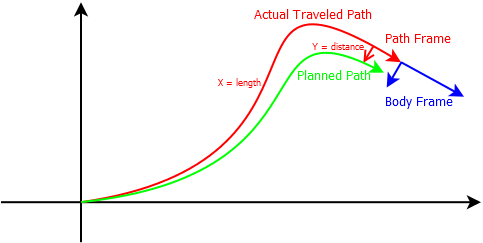
\includegraphics[width = \textwidth]{img/ControlStrategyFigures/PathFrame.png}

\section{Internal Measurement Unit}

We are using an Internal Measurement Unit (IMU) to enhance the estimations and the control system by fusing the velocity data of the \emph{GPS} and the \emph{IMU} based on the accelerometer inputs.
The IMU has the possibility to measure 6 degrees of freedom ($[\ddot{x}, \ddot{y}, \ddot{z}, \dot{Rot_x}, \dot{Rot_y}, \dot{Roz_z}]$). The IMU possesses significantly lower Signal-to-Noise Ratio (SNR) than the GPS velocity measurements. However, using the IMU only for the navigation is ill-considered, because of the small but substantial \emph{bias} of the \emph{Accelerometer} and \emph{Gyro}.
\begin{align}
\hat{x} = x + C(t) = \int \int \ddot{x} dt dt \\
\hat{Rot_x} = Rot_x + C(t) = \int \dot{Rot_x} dt
\end{align}

Therefore we employ a Kalman filter, in order to implement the sensor fusion.

\subsection{Challenges of the IMU signal-processing}

The IMU is fixed to the body of the hull, so if the attitude of the Ship changes, so does the IMU. The data of the three accelerometers can be rotated to a fixed-attitude frame only if we possess the exact attitude data as well. But the attitude data over time will accumulate an unknown amount of offset error, because of (equation No. above).
Since the GPS does not provide any information about the attitude of the ship, another sensor fusion is required, with a fixed outside point, like the Polaris star or the magnetic \emph{North point}.

\subsection{Pitch or roll}

For the control system implementation we employed a simpler solution: assuming the ship will either have no roll or pitch, we could chose to improve either the position estimation or the velocity estimation, based on the natural accelerometer data only.
The \emph{Roll} and the \emph{Pitch} are caused by \emph{perpendicular} and \emph{paralell} external forces attacking the hull of the ship, in respect to the motion.
The measurements during various development phases suggested, that the variance of the fixed GPS position is very low, so enhancing the calculated position based on external forces is not required. In addition we can assume, that the sideways and vertical motion in still water is neglectable.

In the implementation, the sum of the acceleration vectors are calculated, and is compared to a reference gravity acceleration data:
\begin{align}
\sum S = \vec{\ddot{x}} + \vec{\ddot{y}} + \vec{\ddot{z}} \\
F = \arccos{\frac{\sum S}{G}}
\end{align}

In stormy weather the need for a more complex IMU-processing is beyond doubt.